%%%%%%%%%%%%%%%%%%%%%%%%%%%%%%%%%%%%%%%%%%%%%%%%%%%%%%%%%%%%%%%%%%%%%%%%%%%%%%%
% name:         | network.tex
% @uthor:       | Charles Gueunet
% title:        | Include : Le protocole TCP/IP
% brief:        | Explication du protocole TCP/IP
% licence:      | free
% more:         | Warning: inputenc en utf8
%               | Warning: n'oublies pas vos \subsection (3 à 4 maximum)
%%%%%%%%%%%%%%%%%%%%%%%%%%%%%%%%%%%%%%%%%%%%%%%%%%%%%%%%%%%%%%%%%%%%%%%%%%%%%%%


% modele dod : explication de Reseau -> Application
% image modele dod

% Reseau : Ethernet / Bluetooth ...
% Internet : IP addresse (6-4) - ICMP , IGMP
% Transport : Protocol -- TCP / UDP (rapide) - /etc/services  : lien service port protocol
% Application : La donnee, communication noeud à noeud

% Bilan avec image detaillant les headers

\section{Le protocole TCP/IP}
\begin{frame}\frametitle{}
    {\Huge Le protocole TCP/IP}

    \vspace{2em}

    Le net c'est bien, mais comment les machines communiquent ?
\end{frame}


% Presentation du modele DOD dans sa globalité
% Explications rapide des couches (on va revenir dessus en detail en suivant)
% Quelques exemple pour ceux qui connaissent deja
\begin{frame}\frametitle{}
    \subsection{Présentation du modèle DOD}
    {\Huge Présentation du modèle DOD}

    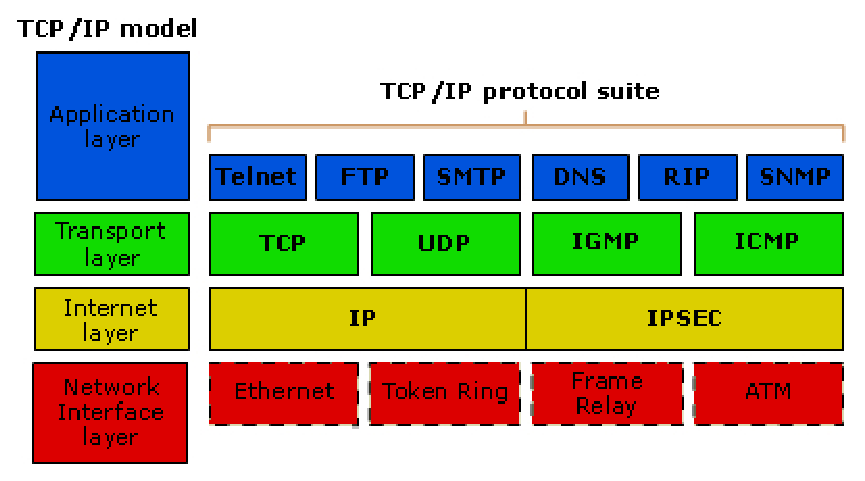
\includegraphics[scale=0.75]{res/DodModel.eps}

\end{frame}


% Couche réseau : Niveau Hardware, la facon dont les 
% donnée sont acheminée entre deux machines
\begin{frame}\frametitle{}
    \subsection{Couche réseau}
    {\Huge Présentation du modèle DOD}

    \begin{itemize}
        \item \textbf{{\Large Couche réseau}: Niveau physique}
    \end{itemize}
     
    % Durant explication : dessin tableau de deux PC relié

\end{frame}


% La couche internet : Interconnexion de reseau (mode déconnecté)
% Sert à l'adressage et au routage des packets
% En d'autre terme l'acheminement de packet à traver plusieurs machines
\begin{frame}\frametitle{}
    \subsection{Couche internet}
    {\Huge Présentation du modèle DOD}

    \begin{itemize}
        \item {\Large Couche réseau}: Niveau physique
        \item \textbf{{\Large Couche internet}: Adressage et routage des packets}
    \end{itemize}

    % Durant explication : dessin tableau de deux PC reliés avec des intermediaires
    % -> Illustre le routage et l'adressage

\end{frame}


%%%%%%%%%%%%%%%%%%%%%%%% EXEMPLE / EXERCICE



% La couche transport : Transmition des données, correction des erreures
% Choix du mode UDP / TCP ( on ne parlera ici que de ces deux la )
% Difference UDP / TCP
\begin{frame}\frametitle{}
    \subsection{Couche transport} % egalement Host to Host layer
    {\Huge Présentation du modèle DOD}

    \begin{itemize}
        \item {\Large Couche réseau}: Niveau physique
        \item {\Large Couche internet}: Adressage et routage des packets
        \item \textbf{{\Large Couche transport}: Transmission des données}
    \end{itemize}

    % Explique succintement les differences TCP/UDP :
    %    TCP         UDP
    % connecté      non connecté
    % ordonné       non ordonné
    % checsum       checksum

\end{frame}


% La couche application : Niveau utilisateur, 
% Echange entre applications
% Choix du protocol à utiliser (généralement TPC/UDP)
\begin{frame}\frametitle{}
    \subsection{Couche application}
    {\Huge Présentation du modèle DOD}

    \begin{itemize}
        \item {\Large Couche réseau}: Niveau physique
        \item {\Large Couche internet}: Adressage et routage des packets
        \item {\Large Couche transport}: Transmission des données
        \item \textbf{{\Large Couche application}: niveau utilisateur}
    \end{itemize}

\end{frame}

% Explication du transit à traver plrs machines
% Utile aussi pour la couche transport
\begin{frame}\frametitle{}
    \subsection{Couche application}
    {\Huge Présentation du modèle DOD}

    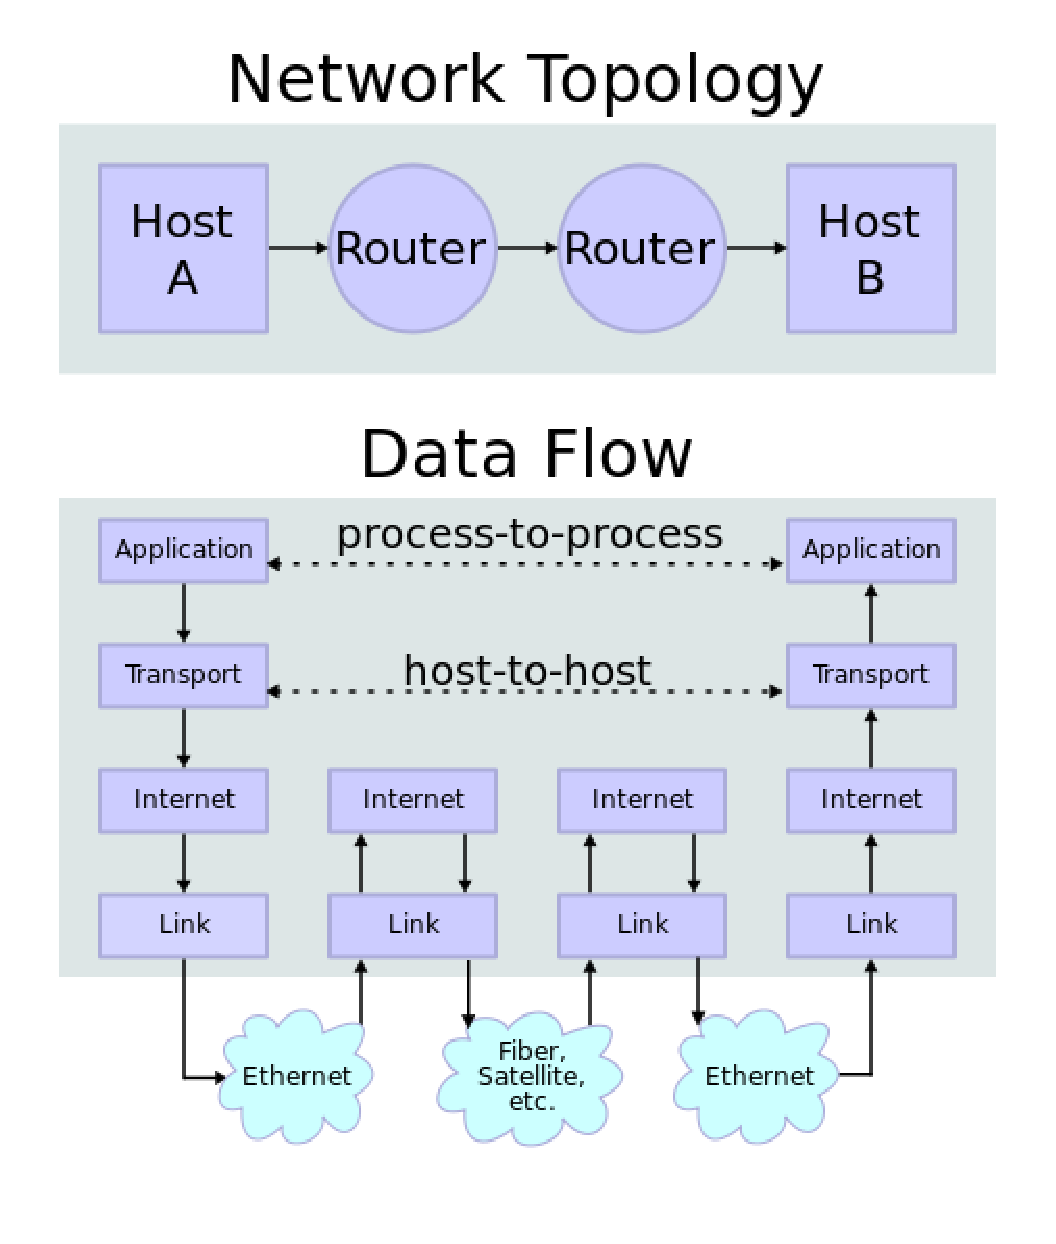
\includegraphics[scale=0.35]{res/DodConnect.eps}

\end{frame}

% On fait un bilan de chaque couche et de leurs interactions
% Conclusion de la partie modele Dod
\begin{frame}\frametitle{}
    \subsection{Bilan du modèle DOD}
    {\Huge Bilan du modèle DOD}

    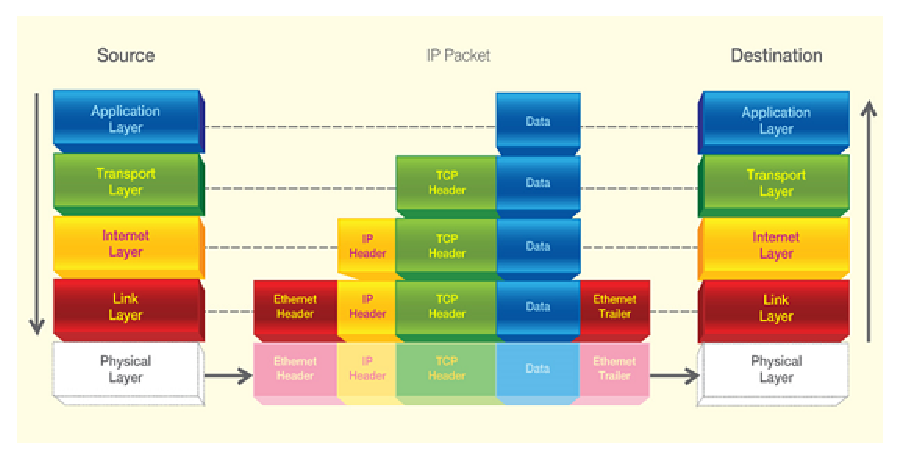
\includegraphics[scale=0.75]{res/DodExplain.eps}

\end{frame}

%% TODO Classes IP 
%% Un TP avec nc : nc -l -p 3333  : Protocol enttec sous wireshark
%% Une Demo avec tcpdump (basé sur les manip du TP)

